\documentclass[12pt]{article}
\usepackage[a4paper, total={7.5in, 11in}]{geometry}
\usepackage{array}
\usepackage{graphicx, subfig, wrapfig, fancyhdr, lastpage, multicol ,color,arydshln,makecell}

\newcommand\headerMe[2]{\noindent{}#1\hfill#2}
\usepackage[mathscr]{euscript}
\usepackage{tabularray}

\setlength{\columnseprule}{1pt}
\def\columnseprulecolor{\color{blue}}


\pagestyle{fancy}
\fancyhf{}

\cfoot{ \vspace{-0.8cm}\em{Page \thepage \hspace{1pt} / \pageref{LastPage}}}
\begin{document}

\headerMe{Royaume du Maroc}{année scolaire \emph{2022-2023}}\\
\headerMe{Ministère de l'Éducation nationale, }{  Professeur :\emph{Zakaria Haouzan}}\\
\headerMe{du Préscolaire et des Sports}{Établissement : \emph{Lycée SKHOR qualifiant}}\\
%\vspace{-1cm}
\begin{center}
Devoir Surveillé  N°2 - S2 \\
    2ème année baccalauréat Sciences physiques\\
Durée 2h00
\\
    \vspace{.2cm}
\hrulefill
\Large{Chimie 7pts - 45min}
\hrulefill\\

    %\emph{Les deux parties sont indépendantes}
\end{center}
%end Headerss------------------------
%__________________Chimie ______________________-
%%%%%%%+_+_+_+_+_+_+_+_+_Partie1

 \section*{Partie 1 : Gaz d’une grande pureté. \dotfill(07pts)- 45min }
\begin{wrapfigure}[5]{r}{0.32\textwidth}
  \begin{center}
	  \vspace{-0.6cm}
	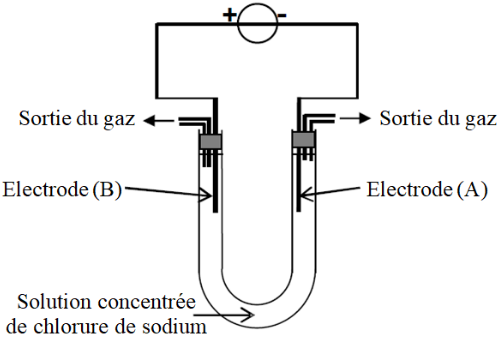
\includegraphics[width=0.32\textwidth]{./img/ex00.png}
  \end{center}
\end{wrapfigure}
	   \emph{L'électrolyse permet d'obtenir des gaz d'une grande pureté.
On réalise l'électrolyse d'une solution concentrée de chlorure de sodium
$Na^+_{(aq)} + Cl^-_{(aq)}$, on obtient un dégagement de dichlore au voisinage de l’une des
électrodes, et dégagement de dihydrogène au voisinage de l'autre électrode, de plus
que le milieu réactionnel \\devient basique au cours de la transformation chimique.}

\begin{itemize}
	\item Les couples intervenants dans la transformation\\ chimique : $(H_2O_{(l)})/H_{(g)})$ et $(Cl_{2(g)}/Cl^-_{(aq)})$
	\item Le faraday $\mathscr{F}=9,65.10^4 C.mol^{-1}$
	\item Le volume molaire dans les conditions de l’expérience :$V_m = 25,0L.mol^{-1}$
\end{itemize}
La figure ci-contre représente le
dispositif expérimental utilisé pour
réaliser cette électrolyse.


\begin{tabular}{c | c}
		1 & \makecell[l]{\textbf{1. }Déterminer laquelle parmi les
électrodes (A) et (B) celle qui
joue le rôle de l'anode et celle\\
qui joue le rôle de la cathode.}\\

			1 & \makecell[l]{\textbf{2. }Ecrire l’équation de la réaction
ayant lieu au voisinage de
chaque électrode, et l'équation\\
bilan de cette électrolyse.}\\

 1 & \makecell[l]{\textbf{3. } Le générateur alimente le circuit avec un courant électrique d'intensité constante
	$I = 3A$.\\Calculer la quantité d’électricité Q débitée au cours de $\Delta{t} = 25 min$. 
}\\

2 & \makecell[l]{\textbf{4. } Calculer le volume du dichlore $Cl_2$ formé pendant la durée $\Delta{t} = 25 min$.}\\
	
2 & \makecell[l]{\textbf{5. } Calculer le volume du dihydrogène $H_2$ formé pendant la durée $\Delta{t} = 80 min$.}\\
\end{tabular}
%\begin{center}
%\begin{tabular}{ |c| c|}
%\hline
%\textbf{Couple acide/base} &\textbf{ Valeur de $pK_A$}\\\hline
	%$HCOOH / HCOO^-$  & 3,75 \\\hline
	%$C_6H_5COOH/C_6H_5COO^-$ &4,2\\\hline
	%$CH_3COOH/CH_3COO^-$&  4,75 \\\hline
	%$CH_3-CH_2-COOH/CH_3-CH_2-COO^-$ &4,9 \\\hline

%\end{tabular}
%\end{center}

%\begin{tabular}{c|l}
	%0,5 & \makecell[l]{\textbf{3. }Déterminer le volume
	%$V_{b1}$ de la solution $S_b$ versée, au cours du dosage, pour que: $\frac{[AH]}{[A^-]} = 2,24$ . }\\
%\end{tabular}

%\hrulefill
%\Large{Physique 13pts/78min}
%\hrulefill\\
%\newpage
\begin{center}
    %\vspace{.60cm}
\hrulefill
\Large{Physique 13pts - 75min}
\hrulefill\\
    %\emph{Les  parties sont indépendantes}
\end{center}

%\vspace{-1cm}
\section*{Exercice 1–un parcours de golf\dotfill(6pts)}

%\begin{wrapfigure}[9]{r}{0.25\textwidth}
  %\begin{center}
	  %\vspace{-1cm}
	%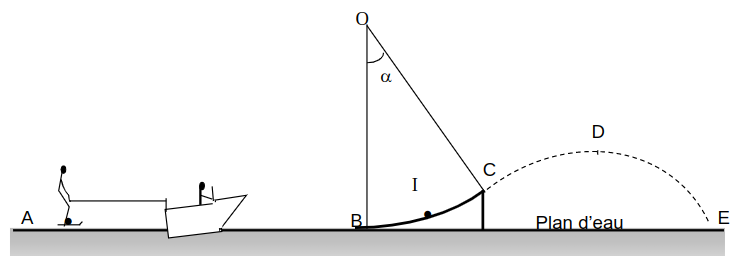
\includegraphics[width=0.19\textwidth]{./img/img01.png}
	%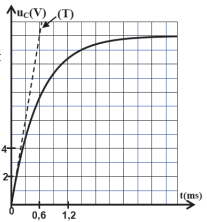
\includegraphics[width=0.25\textwidth]{./img/img02.png}
  %\end{center}
%\end{wrapfigure}

   % \begin{wrapfigure}[7]{r}{0.32\textwidth}
  %\begin{center}

	  %\vspace{-1.6cm}
	%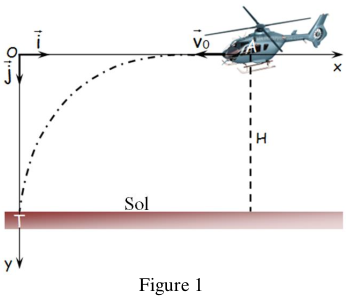
\includegraphics[width=0.32\textwidth]{./img/ex_02.png}
  %\end{center}
%\end{wrapfigure}

La figure ci-dessous schématise un parcours de golf. Le joueur désire envoyer la balle dans le trou
(drapeau) situé derrière un arbre d’une hauteur de $12 m$.

Le joueur, communique à la balle une vitesse initiale $V_0$ dont la direction du vecteur fait un angle $\alpha$
avec l’horizontale passant par l’origine de lancement. (figure 3 ci dessous) .

On suppose que les forces exercées par l'air sur la balle sont négligeables.



 \begin{center}
	  %\vspace{-1cm}
	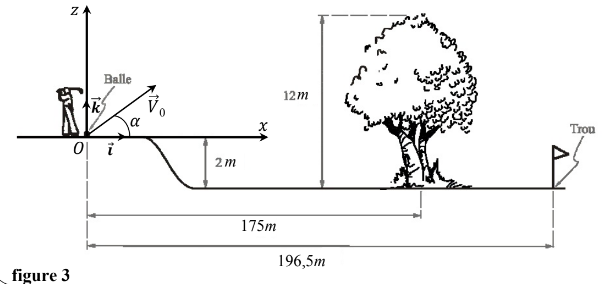
\includegraphics[width=0.8\textwidth]{./img/chute00.png}
  \end{center}


On étudie le mouvement de la balle dans le champ de pesanteur uniforme dans un repère orthonormé
$(O,\vec{i} , \vec{k})$ lié à la Terre considéré galiléen.

\begin{tabular}{c|l}	
	1 & \makecell[l]{\textbf{1. }En appliquant la deuxième loi de newton, déterminer les équations différentielles vérifiées \\par les
coordonnées $V_x$ et $V_z$ du vecteur vitesse de la balle dans le repère $(O, \vec{i} , \vec{k})$.}\\
	1 & \makecell[l]{\textbf{2. }Établir les équations horaires du mouvement $x(t)$ et $z(t)$. }\\
	0,75 & \makecell[l]{\textbf{3. }Vérifier que l’équation de la trajectoire s’exprime:$z = \frac{-g}{2.V_0^2.cos^2\alpha}.x^2 + xtan\alpha$ }\\
	0,75 & \makecell[l]{\textbf{4. }Les courbes de la figure 4 représentent les variations de $V_x$
et $V_z$
en fonction du temps\\ Vérifier que  : $v_0 \approx 46,04 m.s^{-1}$ et que $\alpha \approx 32,86^{\circ}$}\\
	1 & \makecell[l]{\textbf{5. }En déduire la valeur de g l’intensité de la pesanteur. }\\
	0,75 & \makecell[l]{\textbf{6. }Montrer que la balle passe au dessus de l’arbre. }\\
	0,75 & \makecell[l]{\textbf{7. }Est ce que le joueur a réalisé son objectif ?. }\\
\end{tabular}


 \begin{center}
	  %\vspace{-1cm}
	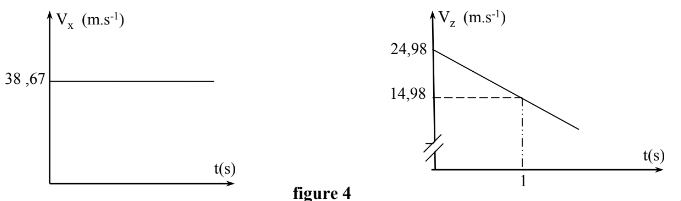
\includegraphics[width=0.8\textwidth]{./img/chute__01.png}
  \end{center}



\section*{Exercice 2–Mouvement d’une particule chargée \dotfill(2,5pts)}


	\begin{wrapfigure}[4]{r}{0.2\textwidth}
  \begin{center}
	  \vspace{-0.8cm}
	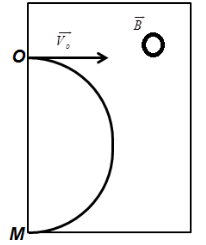
\includegraphics[width=0.2\textwidth]{./img/ex_00.png}
  \end{center}
\end{wrapfigure}

Les ions $O^{-}$ pénètrent dans une région de l'espace où règne un champ $\vec{B}$(perpendiculaire au plan de la figure). Avec une vitesse
magnétique uniforme  $V_0 =1,6.10^4.m.s^{-1}$

\textbf{Données :} L'intensité du champs magnétique $B= 0,1T$ ; La charge élémentaire $e = 1, 6.10^{-19} C$



\begin{tabular}{c|l}	

1	  & \makecell[l]{\textbf{1. }Donner les caractéristiques de la force magnétique $\vec{F_m}$.
}\\
	0,25 & \makecell[l]{\textbf{2. }Déterminer le sens du champs magnétique $\vec{B}$.
 }\\
	0,75 & \makecell[l]{\textbf{3. }En appliquant la deuxième loi de newton dans un référentiel galiléen,
		\\montrer que le mouvement des ions $O^{-}$ est circulaire uniforme.}\\
	 0,5& \makecell[l]{\textbf{4. }Calcule la masse d'ion $O^{-}$ (On donne $OM = 4 cm$ )
}\\
\end{tabular}

\newpage
\section*{Exercice 3 – Mouvement des satellites et planètes \dotfill(4,5pts)}

On suppose que la Terre, de masse $M_T$ , de rayon $R_T$ et de centre O, est une sphère et qu'elle présente une répartition de masse à symétrie sphérique. Un satellite artificiel S, de masse $m_S$ , décrit une orbite circulaire de rayon r autour de la Terre (figure 1).

On néglige toutes les forces exercées sur le satellite S devant la force
d’attraction universelle exercée par la Terre ainsi que les dimensions
de S devant la distance qui le sépare du centre O de la Terre.

\begin{center}
	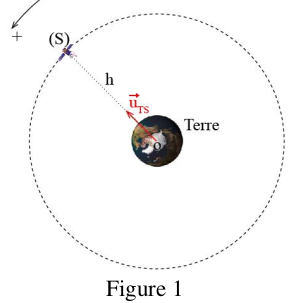
\includegraphics[width=0.26\textwidth]{./img/ex__00 .png}
  \end{center}


\textbf{On donne : }
la constante de gravitation universelle $G =6,67.10^{-11} (SI)$

\begin{tabular}{c|l}	

	0,5  & \makecell[l]{\textbf{1. }Exprimer l’intensité du champ de gravitation terrestre $g_h$ en fonction de $M_T$, $R_T$, h et G.}\\
	1  & \makecell[l]{\textbf{2. }Montrer que le mouvement du satellite dans le référentiel
géocentrique est circulaire uniforme.}\\

	 1 & \makecell[l]{\textbf{3. }En déduire l'expression de la vitesse v du satellite en fonction de G, $M_T$ et r puis celle de sa \\période T de révolution.}\\

	   & \makecell[l]{\textbf{4. } Le tableau suivant rassemble les valeurs numériques des périodes de révolution T et \\ des rayons r des orbites de quelques satellites artificiels de la Terre.}\\
\end{tabular}
\begin{center}
\begin{tabular}{ |c| c| c|c|c| }
	\hline
	Base de lancement & Kourou & Baïkonour & Chine & Etats-Unis\\\hline
	Satellite & Intelsat-V & Cosmos-197 & Feng-Yun & USA-35 \\\hline  
	r ($10^4$ km) & 4,22 & 2,55 & 0,73 & 2,66\\\hline
	
\end{tabular}

\end{center}


\begin{tabular}{c|l}	

	1  & \makecell[l]{\textbf{4.1. }Vérifier, à partir des valeurs numériques du tableau, que le rapport$\frac{T^2}{r^3}$  est \\une constante que l’on déterminera.}\\

	1  & \makecell[l]{\textbf{4.2. }calculer la masse $M_T$ de la Terre. }\\
\end{tabular}
\end{document}
